\documentclass{st50_template}
\usepackage{listings}
\usepackage{xcolor}
\lstdefinestyle{sharpc}{language=[Sharp]C}
\lstset{style=sharpc}
\begin{document}
\sffamily
\thispagestyle{empty}
\begin{picture}(0,0)
%Images
\put(-90, -130){
\includegraphics[scale=0.897]{images/image_fond}}
\put(380, -708){
\includegraphics[scale=0.897]{images/logo_UTBM}}
%Color
\put(-89, -148){\colorbox{black}{\makebox(609, 15){}}}
\put(-89, -234){\colorbox{purple}{\makebox(609, 80){}}}
\put(-89, -255){\colorbox{gray}{\makebox(609, 15){}}}
\put(-89, -641){\colorbox{yellow}{\makebox(609, 380){}}}
%Text
\put(-72, -146){\Large\textcolor{white}{\textbf{UNIVERSITÉ DE TECHNOLOGIE} DE BELFORT-MONTBÉLIARD}}
\put(-72, -201){\Huge\textcolor{white}{Serious game de rééducation}}
\put(-72, -251){\large\textcolor{white}{Rapport de IN52 - IN54}}
\put(-72, -296){\Large{\textbf{BOUCHEREAU Thomas - BRUNET Pierre - PERREZ Stéphane}}}
\put(-62, -316){\large\textcolor{gray}{Département Informatique - Imagerie, Interaction et Réalité Virtuelle}}
%\put(-42, -426){\Large{\textbf{LABORATOIRE SYSTEMES ET TRANSPORTS (IRTES SET)}}}
\put(-62, -416){\large\textcolor{gray}{Université de Technologie de Belfort Montbéliard}}
\put(-62, -431){\large\textcolor{gray}{90 010 - BELFORT CEDEX}}
\put(-72, -576){\large\textcolor{gray}{\textbf{Responsable TX52}}}
\put(-72, -596){\Large{\textbf{GECHTER Frank}}}
\put(320, -576){\large\textcolor{gray}{\textbf{Enseignant VI50}}}
\put(320, -596){\Large{\textbf{CHEVRIAU Sébastien}}}
\end{picture}

\newpage
\thispagestyle{empty}
\tableofcontents

\newpage

\section{Objectifs du projet}

Le but du projet est de faire de la reconnaissance de jeux de plateaux à partir de leur boîte de jeu et d'une base de données. Il nous faut donc procéder en plusieurs étapes. Ainsi, nous devons recentrer la photo sur la face du dessus puis la recadrer afin d'avoir la meilleure analyse possible. Ensuite, nous allons comparer le pourcentage de couleur entre les jeux de la base de données et la photo. Cette base de données est censée se créer au fur et à mesure à l'aide d'une interface.

Nous avons décidé de diviser le projet en trois parties. Ainsi, le premier étudiant s'occuperait du recadrage de la face du dessus de la boîte. Le second prendrait en charge la comparaison de deux images données. Enfin, le dernier créerait la base de données et l'interface graphique afin que l'application soit utilisable en dehors de tests divers.


\section{Développement}

\subsection{Récupérer la face du dessus de la boîte de jeu}
Pour récupérer la face du dessus, il est nécessaire de pouvoir distinguer les contours dans l'image. Nous avons donc décidé d'utiliser la transformée de Hough pour cela. Mais avant tout, il nous faut enlever le bruit de l'image afin d'éviter des contours inutiles. Nous avons donc utiliser la technique d'érosion puis avons rogner l'image en fonction de la densité restante dans les lignes de l'image.

\begin{figure}[ht]
    \centering
    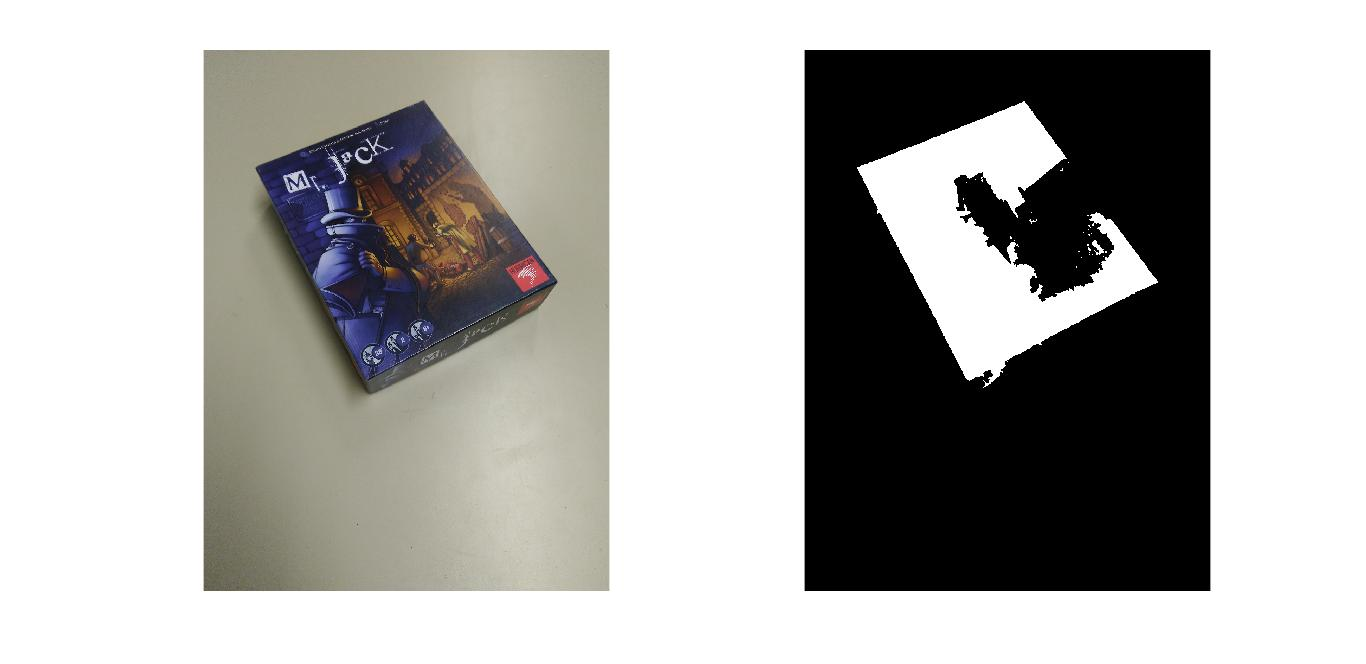
\includegraphics[width=0.77\textwidth]{images/erosion.jpg}
    \caption{Image binaire et érodée}
    \label{erosion}
\end{figure}

\begin{figure}[ht]
    \centering
    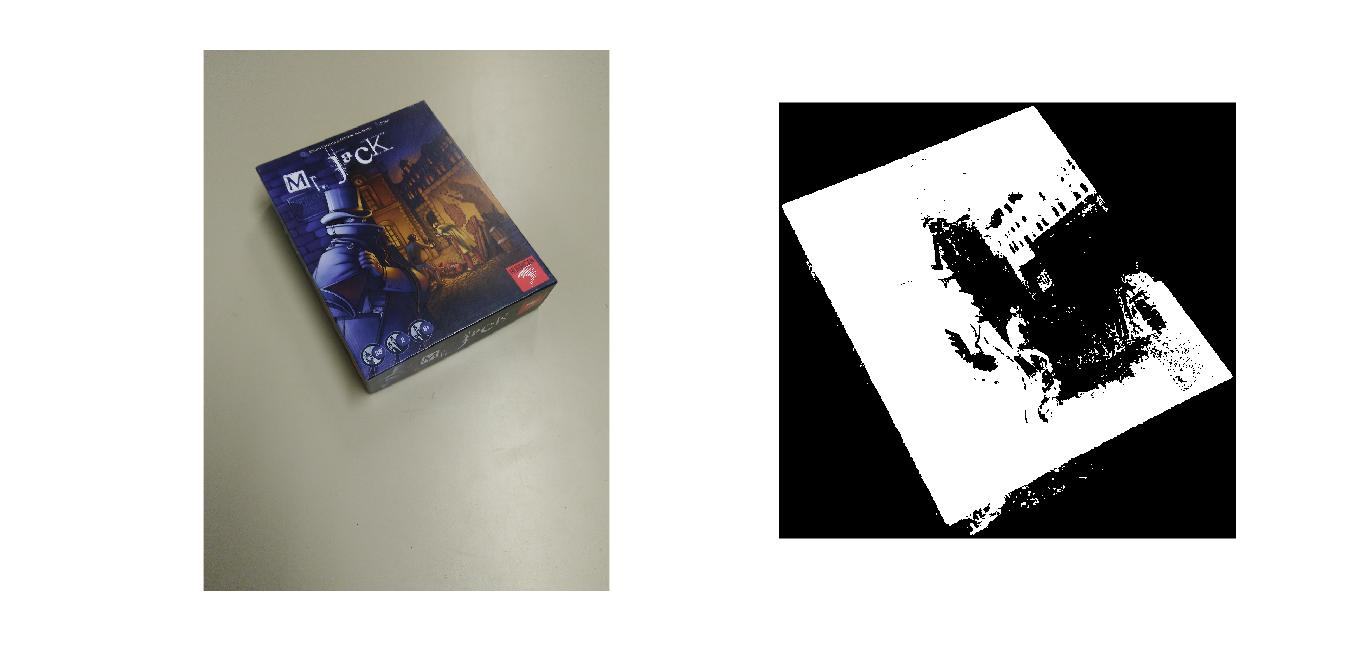
\includegraphics[width=0.77\textwidth]{images/rognage.jpg}
    \caption{Image binaire rognée}
    \label{rognage}
\end{figure}

Après ce pré-traitement, on applique la transformée de Hough à des lignes faisant au moins une certaines longueur pour éviter d'avoir des lignes du dessin du jeu. On allonge ensuite ces lignes et on récupère les points d'intersection. 

Ces points d'intersection ont été produits grâce aux fonctions \emph{polynomes} et \emph{polyval}. Cependant, les lignes générées ne sont pas forcément dans le bon ordre. Par conséquent, les points ne le sont pas non plus. De plus, on génère toutes les intersections de lignes possibles. Il faut donc faire un tri pour éviter les duplicas et également les trier dans un ordre donné. C'est le dernier traitement que j'applique avant de passer à l'analyse de l'image.

\begin{figure}[ht]
    \centering
    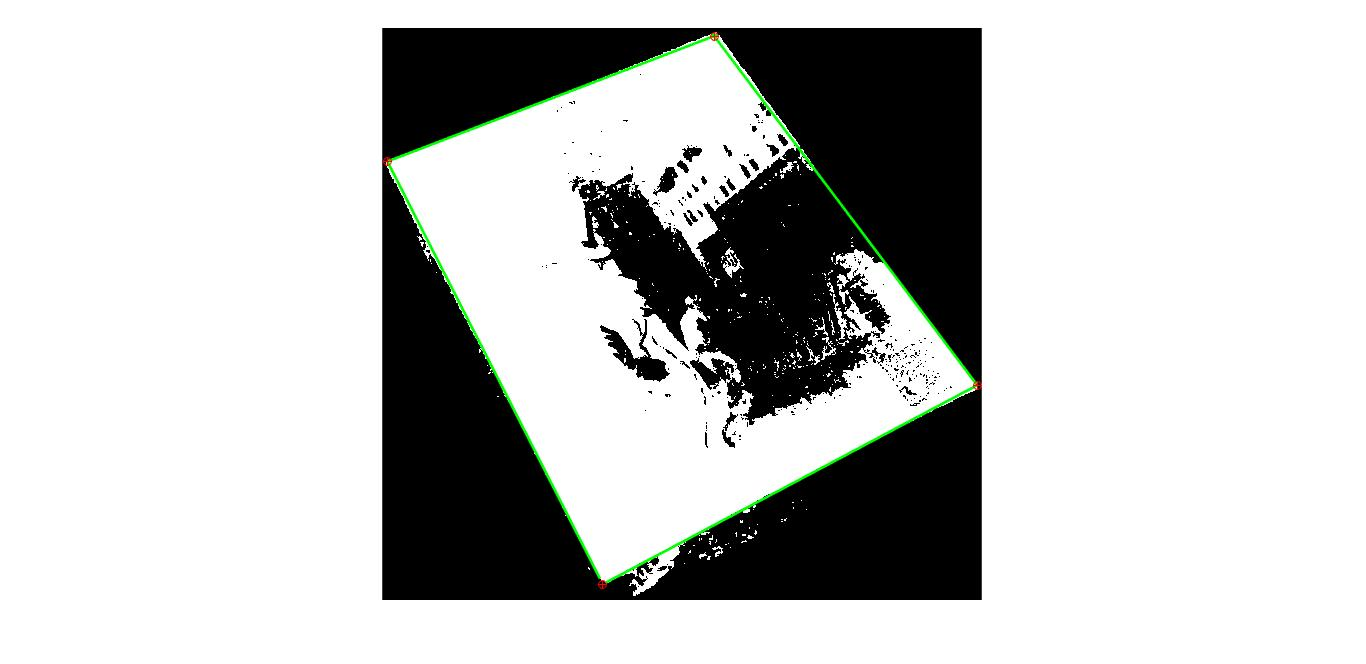
\includegraphics[width=0.77\textwidth]{images/contourEtPts.jpg}
    \caption{Contours de la face du dessus}
    \label{contourEtPts}
\end{figure}

\subsection{De la 3D à la 2D}
Une fois les points récupérés, il nous faut adapter l'image pour la rendre comparable avec l'image de base. On utilise donc les points d'intersection précédemment calculés.

La fonction fitgeotrans permet de rapprocher une image d'une autre grâce à un tableau de points mouvants et un tableau de points fixes. Le tableau de points mouvants doit \emph{rentrer dans} (\emph{fit} en Anglais) le tableau de points fixes.

\begin{figure}[ht]
    \centering
    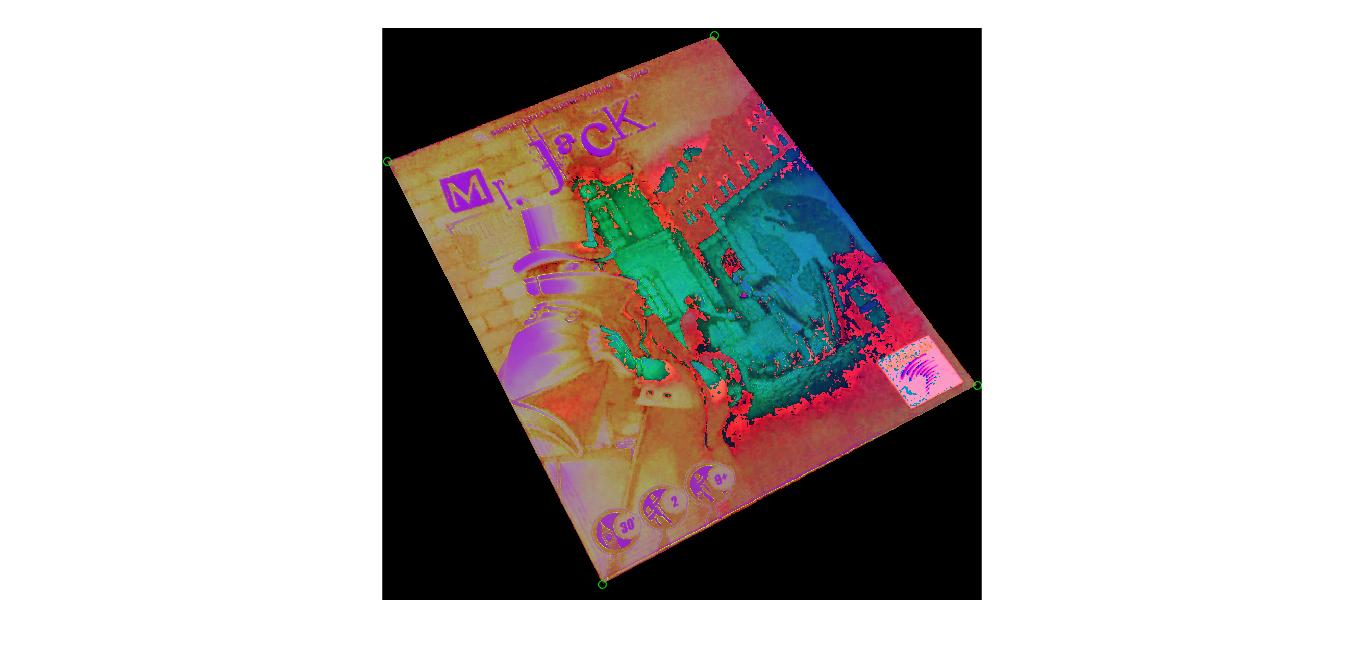
\includegraphics[width=0.77\textwidth]{images/movingPoints.jpg}
    \caption{Points mouvants en vert sur l'image}
    \label{movingPoints}
\end{figure}


C'est à partir de ce moment-là que nous avons rencontré des problèmes. En effet, la fonction n'est pas aussi efficace qu'elle le sous-entend. Malgré tous nos efforts, nous n'avons pu que redresser la boîte sans pouvoir changer les angles de l'image.

Vous verrez sur les figures \ref{fitgeotrans} et \ref{transRecadre} les différents résultats obtenus grâce à la fonction Matlab fitgeotrans.

\begin{figure}[ht]
    \centering
    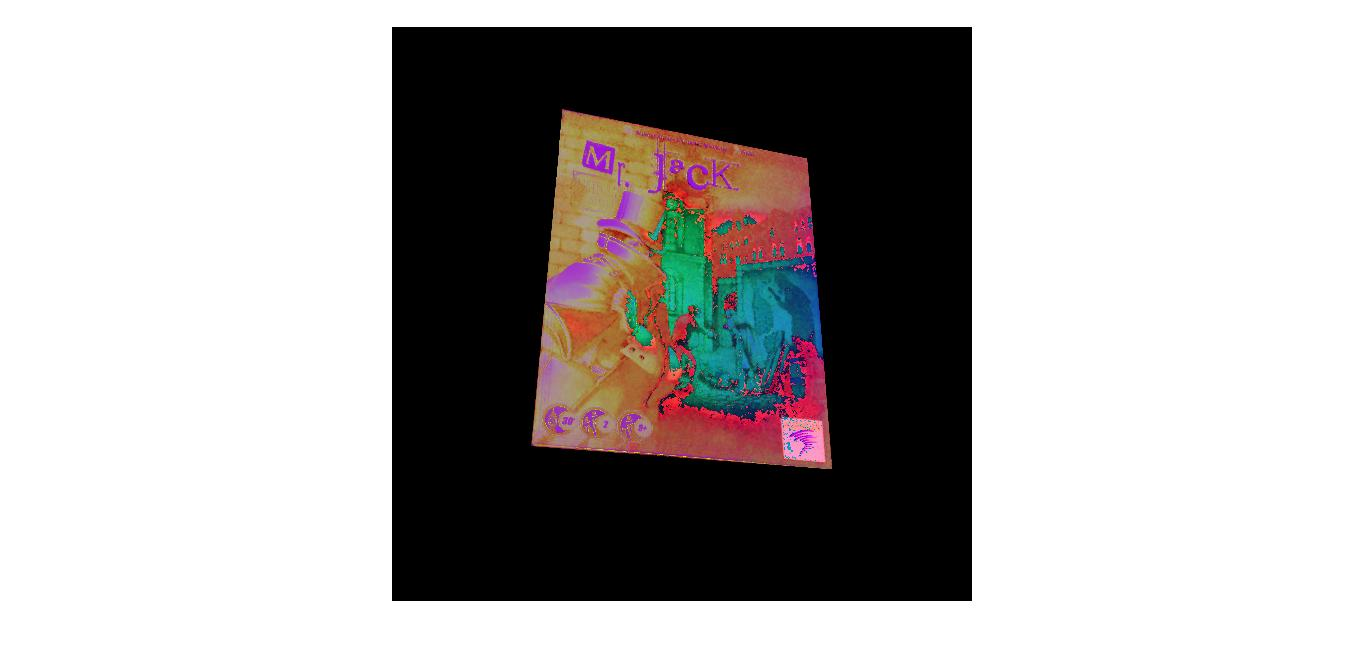
\includegraphics[width=0.77\textwidth]{images/fitgeotrans.jpg}
    \caption{Résultat de la fonction \emph{fitgeotrans}}
    \label{fitgeotrans}
\end{figure}

\begin{figure}[ht]
    \centering
    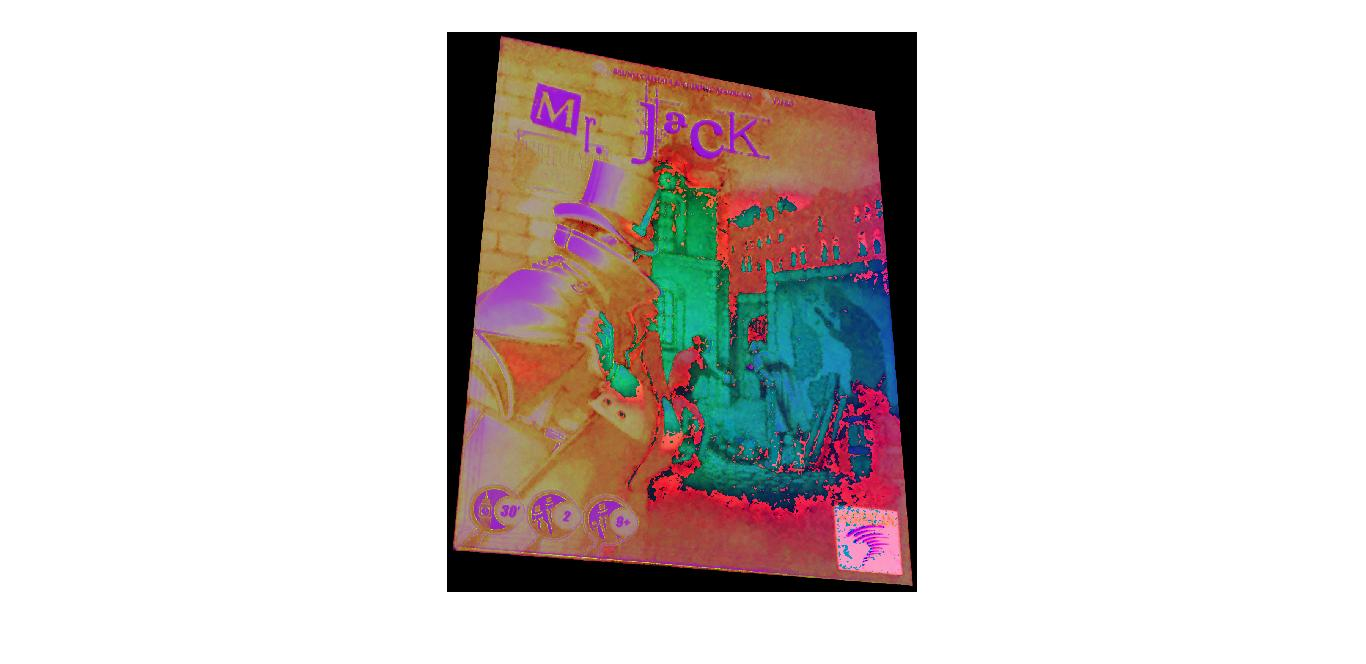
\includegraphics[width=0.77\textwidth]{images/transRecadre.jpg}
    \caption{Recadrage maximal obtenu}
    \label{transRecadre}
\end{figure}

\subsection{Analyse des fréquences}

Nous avons donc décidé de revenir à l'image pré-traitée et ne comparer que les fréquences de couleurs afin de pouvoir rapidement reconnaître un jeu. Cela s'est révélé plus logique et plus optimisé en prenant comme couleurs le HSL. Nous n'avions alors qu'à récupérer le Hue (à savoir la nuance) de chaque pixel et comparer les densités par rapport à la base de données.

\subsection{Apprentissage}

\section{Conclusion}
\end{document}